\documentclass[spanish,notitlepage,letterpaper,11pt]{article} % para
                                % articulo en castellano
\usepackage[utf8]{inputenc}
%\usepackage[ansinew]{inputenc} % Acepta caracteres en castellano
\usepackage[spanish]{babel}    % silabea palabras castellanas
\usepackage{amsmath}
\usepackage{amsfonts}
\usepackage{amssymb}
\usepackage[colorlinks=true,urlcolor=blue,linkcolor=blue]{hyperref} % navega por el doc
\usepackage{graphicx}
\usepackage{geometry}           % See geometry.pdf to learn the layout options.
\geometry{letterpaper}          % ... or a4paper or a5paper or ... 
%\geometry{landscape}           % Activate for for rotated page geometry
%\usepackage[parfill]{parskip}  % Activate to begin paragraphs with an empty line rather than an indent
\usepackage{epstopdf}
\usepackage{fancyhdr} % encabezados y pies de pg
\pagestyle{fancy} 
\chead{} 
%\lhead{\textit{ Encabezado izquierdo }} % si se omite coloca el nombre de la seccion
%\rhead{\textbf{Encabezado derecho}} 
%\rfoot{\thepage} 

\voffset = -0.25in 
\textheight = 8.0in 
\textwidth = 6.5in
\oddsidemargin = 0.in
\headheight = 20pt 
\headwidth = 6.5in
\renewcommand{\headrulewidth}{0.5pt}
\renewcommand{\footrulewidth}{0,5pt}

\newcommand{\apj}{ApJ}
\newcommand{\apjs}{ApJS}
\newcommand{\apjl}{ApJL}
\newcommand{\aj}{AJ}
\newcommand{\mnras}{MNRAS}
\newcommand{\mnrassub}{MNRAS accepted}
\newcommand{\aap}{A\&A}
\newcommand{\aaps}{A\&AS}
\newcommand{\araa}{ARA\&A}
\newcommand{\nat}{Nature}
\newcommand{\prd}{PRD}
\newcommand{\physrep}{PhR}
\newcommand{\pasp}{PASP}
\newcommand{\pasj}{PASJ} 

\begin{document}


\section*{}
\begin{center}
{\LARGE T\'itulo del proyecto: \\ {\bf Cosmolog\'ia Computacional y Observacional}}
\end{center}

%
\section*{}
\begin{center}
{\LARGE Investigador Principal }\\
{\LARGE \textbf{Jaime Ernesto Forero Romero} \\ 
\textit{Grupo de Investigación en Astrof\'isica, C\'odigo COL0015473} \\
\textit{Departamento de Física, Facultad de Ciencias, }\\
\textit{Universidad de los Andes, Bogot\'a-Colombia}}
\end{center}




\newpage 
\tableofcontents 
\section{Conformaci\'on del equipo de investigaci\'onn}
%Colocar el nombre y código, registrado en el GrupLac, del o de los
%grupos de investigación. Al igual que el nombre de los demás
%integrantes que conforman el equipo de trabajo. Se debe incluir el
%tiempo de dedicación y funciones en el marco del proyecto.  

La investigaci\'on se har\'a dentro del grupo de astrof\'isica de la
Universidad de los Andes, c\'odigo GrupLAC COL0015473. Los integrantes
del equipo son los siguientes. 


\begin{itemize}
\item Un profesor de planta del grupo de Astrof\'isica de la
  Universidad de los Andes: Jaime Ernesto  Forero Romero, PhD.
  Dedicaci\'on: 7 horas/semana.
\item Dos estudiantes de doctorado en el departamento de F\'isica de
  la Universidad de los Andes.
\begin{itemize}
\item Felipe Leonardo G\'omez Cort\'es
  (F\'isico) con participaci\'on activa en los 36 meses del proyecto. Dedicaci\'on: 20 horas / semana.  
  \item Estudiante por definir con participaci\'on activa en los 24 \'ultimos
    meses del proyecto (los primeros 12 estar\'an enfocados a
    actividades formativas).  Dedicaci\'on: 20 horas / semana.  
\end{itemize}
\end{itemize}

\noindent
Con el apoyo de los siguientes asesores internacionales:

\begin{itemize}

\item Stefan Gottloeber, PhD. Cient\'ifico en el Leibniz Institute for
  Astrophysics, Alemania.  
\item Changbom Park, PhD. Miembro permanente del Korean Institute for
  Advanced Studies, Corea del Sur. 
\item Robert Cahn, PhD. Cient\'ifico en el Lawrence Berkeley National
  Laboratory, Estados   Unidos. 
\end{itemize}

\noindent
Adicionalmente el proyecto cuenta con el soporte del siguiente
personal t\'ecnico de la Universidad de los Andes:

\begin{itemize}
\item{Ingeniero de c\'omputo del departamento de F\'isica.}
\item{Ingeniero de c\'omputo de alto rendimiento en el Direcci\'on de
  Servicios de Informaci\'on y Tecnolog\'ia.}
\end{itemize}

\section{Antecedentes y resultados previos del equipo de
  investigaci\'on} 
%  investigación solicitante en la temática específica del proyecto} 
% trayectoria del equipo de investigación con relación al problema
% planteado en el proyecto. 

El l\'ider del equipo de investigaci\'on tiene un PhD en el \'area de
simulaciones de formarci\'on de galaxias en un  contexto
cosmol\'ogico, 5 a\~nos de experiencia postdoctoral en el tema (en
Alemania y Estados Unidos) y 2 a\~nos de trabajo como
investigador/profesor en el grupo de  Astrof\'isica de la Universidad
de los Andes. 


Adicionalmente durante el \'ultimo a\~no, se ha involucrado en dos
colaboraciones internacionales: 

\begin{itemize}
\item Con el experimento DESI
(Dark Energy Spectroscopic Instrument) liderado por el Lawrence
Berkeley National Laboratory en Estados Unidos
(\url{http://desi.lbl.gov/}). 
Esta colaboraci\'on medir\'a el efecto
de la energ\'ia oscura en la historia de expansi\'on del
Universo. 
DESI medir\'a los espectros de cerca de 20 millones de galaxias
para crear un mapa 3D del Universo con  profundidad de 10mil
millones de a\~nos luz. 
El contacto principal de Jaime Forero en esta colaboraci\'on desde
comienzos del 2014 es el Dr. Robert Cahn, con quien se han venido
desarrollando trabajos para la prepraci\'on del experimento que
empezar\'a a tomar datos en el 2018. 

\item Con el equipo de Cosmolog\'ia del Korean Institute for Advanced
  Studies (KIAS) (\url{http://www.kias.re.kr/}). 
Esta colaboraci\'on se centra en el desarrollo de nuevos 
  algoritmos para acotar los par\'ametros cosmol\'ogicos a trav\'es de
  mediciones de la distribuci\'on de galaxias a gran escala. 
  El contacto principal en esta colaboraci\'on desde mediados del 2013 es
  el Dr. Changbom Park. 
  Un aspecto atractivo de esta colaboraci\'on es
  la posibilidad de aplicar estos algoritmos sobre datos observacionales del
  SDSS-III (Sloan Digital  Sky Survey) (\url{https://sdss3.org/}) en
  el periodo en el que todav\'ia no son p\'ublicos los  datos, gracias
  al que KIAS hace parte de la colaboraci\'on SDSS. 

\end{itemize}

En los \'ultimos 5 a\~nos, el lider del grupo se ha dedicado a
investigar y publicar en el tema. En los temas relevantes para esta
propuesta sobresalen las siguientes publicaciones:

\noindent
En el tema de simulaciones y evoluci\'on de estructura a gran escala:

\begin{itemize}

\item {\it Cosmic web alignments with the shape, angular momentum and
  peculiar velocities of dark matter halos} {\bf Forero-Romero} J.E.,
  Contreras S., Padilla N., Accepted for publication in MNRAS,
  arXiv:1406.0508.

\item{\it The velocity shear tensor: tracer of halo alignment},
  Libeskind N., Hoffman Y., {\bf Forero-Romero} J.E., Gottloeber S.,
  Knebe A., Steinmentz M., Klypin A., MNRAS 428, 2489, 2013 

\item
{\it The dark matter assembly of the Local Group in constrained cosmological
  simulations of a $\Lambda$CDM universe} {\bf Forero-Romero} J.E., Hoffman Y., Yepes G., Gottl\"ober S.,
  Piontek R., Klypin A., Steinmetz M., 
MNRAS, 417, 1434, 2011

\item
{\it Halo based reconstruction of the cosmic mass density field}
Mun\~oz-Cuartas J. C., M\"uller V, {\bf Forero-Romero} J. E., MNRAS,
417, 1303, 2011  

\item
{\it A Dynamical Classification of the  Cosmic Web}.  {\bf
  Forero-Romero} J.E., Hoffman Y.,  Gottloeber S., Klypin A., Yepes G., MNRAS, 396, 1815-1824, 2009 

\item 
{\it The coarse geometry of merger trees in
  $\Lambda$CDM}.  {\bf Forero-Romero} J.E., 
MNRAS, 399, 762-768, 2009

\end{itemize}

\noindent
En el \'area de utilizar eventos extremos como prueba cosmol\'ogica:

\begin{itemize}
\item{\it The abundance of Bullet Groups in $\Lambda$CDM},
  J. G. Fern\'andez-Trincado, {\bf J. E. Forero-Romero}, G. Foex,
  V. Motta, T. Verdugo, V. Motta, ApJ Letter, 787, L32, 2014.
\item
{\it Bullet Clusters in the MareNostrum Universe}. 
{\bf Forero-Romero} J.E., Yepes G., Gottl\"ober S., 
ApJ, 725, 1, 2010.
\end{itemize}


\noindent 
En el \'area de analizar datos de simulaciones cosmol\'ogicas
para hacerlas disponibles a la comunidad acad\'emica:

\begin{itemize}
\item{\it The MultiDark Database: Release of the Bolshoi and
  MultiDark Cosmological Simulations} , K. Riebe , A. M. Partl,
  H. Enke, {\bf J.E. Forero-Romero}, S. Gottloeber, A. Klypin,
  G. Lemson, F. Prada, J. R. Primack, M. Steinmetz, V. Turchaninov,
  Astronomische Nachrichten, 334, 691, 2013. 
\end{itemize}




\section{Tem\'atica de investigaci\'on}
% Especificar en cuál de las temáticas definidas por la convocatoria
% está enmarcado el proyecto. 




\section{Resumen ejecutivo}
% Información mínima necesaria para comunicar de manera precisa los
% contenidos y alcances del proyecto. 

La {\bf cosmología observacional} entró en una época dorada con la medición
de las anisotropías de la radiación cósmica de fondo (Premio Nobel de
Física 2006) y la medición de la expansión acelerada del Universo
(Premio Nobel de Física 2011). 

Hoy en d\'ia una de las fronteras de la investigación en cosmología
observacional es la obtenci\'on de mejores mediciones de la historia de
expansión acelerada del Universo.
El objetivo de estas mediciones es restringir los  modelos de la
llamada Energ\'ia Oscura, posible responsable de este efecto. 
Una de las t\'ecnicas observacionales que se utiliza con ese
prop\'osito es la detecci\'on del pico de Oscilaciones Ac\'usticas de
Bariones (OAB) que requiere la medici\'on de las \emph{posiciones} de
millones de galaxias \cite{Eisenstein2005}. 
Otros m\'etodos usan informaci\'on sobre las \emph{velocidades}
peculiares (i.e. velocidades que no es\'an asociadas al flujo de
Hubble) de las galaxias y las distorsiones que estas generan en las
observaciones para cuantificar el crecimiento de estructura a gran
escala \cite{Scoccimarro2004}. 

Las {\bf simulaciones computacionales} juegan un rol central en estos
esfuerzos observacionales para medir el Universo.
Las simulaciones son necesarias para traducir las premisas te\'oricas
en cantidades observables. 
Es decir, son un puente entre la teor\'ia y
la  observaci\'on. 
Hoy en d\'ia,  las simulaciones tambi\'en sirven para preparar una
nueva campa\~na observacional.  
El objetivo es simular todo antes de empezar a medir. 


{\bf La presente propuesta tiene como objetivo hacer investigaci\'on en
Cosmolog\'ia Computacional como fundamento de actividades en
Cosmolog\'ia Observacional.}

En el frente de cosmolog\'ia computacional proponemos realizar una serie de
simulaciones de la distribuci\'on de materia en el Universo a gran
escala sin precedentes en el pa\'is. 
Para la preparaci\'on de estas simulaciones haremos uso de las
m\'aquinas de las Instalaciones para C\'omputo de Alto Rendimiento de
la Universidad de los Andes, las cuales ser\'an instaladas y puestas
en funcionamiento durante el segundo semestre del 2014.

Vamos a usar estas simulaciones de manera principal para fundamentar
nuestro trabajo en Cosmolog\'ia Observacional en dos colaboraciones
internacionales. 

La primera colaboraci\'on, con el Lawrence Berkeley National Laboratory,
se trata de contribuir en la preparaci\'on del experimento DESI (Dark
Energy Spectroscopic Instrument). 
DESI es una colaboraci\'on internacional de m\'as de 100 cient\'ificos
que construir\'a el experimento de siguiente generaci\'on para medir
la historia de expansi\'on del Universo haciendo un mapa de la
distribuci\'on de 25 millones de galaxias, 10 veces m\'as de lo que ha
sido observado hasta la fecha \cite{DESI2013}. 
En particular, esperamos durante la duraci\'on del presente proyecto
con COLCIENCIAS aportar al dise\~no y optimizaci\'on de la estrategia
de las observaciones.  

La segunda colaboraci\'on, con el Korean Insitute for Advanced Studies
(KIAS), trata de la la restricci\'on de par\'ametros cosmol\'ogicos a
partir de la anisotrop\'ia de la distribuci\'on de galaxias. 
En una primera etapa esperamos usar las simulaciones para optimizar los
m\'etodos estad\'isticos de medici\'on del efecto buscado. 
En una segunda etapa vamos a aplicar este conocimiento sobre los datos
observacionales del proyecto SDSS-III (Sloan Digital Sky Survey),
algo posible gracias a la participaci\'on de KIAS en ese proyecto.

Los proyectos posibles con la serie de simulaciones que vamos a
realizar abren la puerta a otro tipo de estudios sobre la estructura
del Universo a gran escala \cite{Tweb,Vweb} y la cuantificaci\'on de
la abundance eventos de colisiones extremas en el Universo
\cite{Bullets2010,Bullets2014}. 
Adicionalmente, estos datos se har\'an disponibles a toda la comunidad
(colombiana e internacional) para realizar diferentes tipos de
estudios y an\'alisis \cite{Multidark}.  
En el curso de este proyecto tambi\'en vamos a organizar una escuela
internacional de un mes, con expertos internacional, para formar
investigadores en Colombia y en la regi\'on andina que est\'enn en capacidad de
utilizar recursos computacionales avanzados para resolver problemas en
cosmolog\'ia computacional y observacional.




\section{Palabras clave}
% Incluir máximo seis (6) palabras clave que describan el objeto del
% proyecto. 

Astrof\'isica --- Cosmolog\'ia --- Materia oscura --- Energ\'ia oscura
--- Estructura a gran escala --- Computaci\'on de alto rendimiento 



\section{Planteamiento del problema}
% Delimitación clara y precisa del objeto de la investigación que
% se realiza por medio de una pregunta.

La pregunta que dirige la investigaci\'on de este proyecto es: ¿Cómo
se estructura el Universo en el que vivimos?

Nuestro objetivo principal es cuantificar la influencia de diferentes
par\'ametros cosmol\'ogicos sobre la formaci\'on estructura en el Universo.
Para esto haremos simulaciones de la evolución de estructuras en
grandes escalas lo que nos permitirá poner pie en una colaboración
internacional que busca observar lo que hemos simulado en la
computadora.

Para entender esta perspectiva de trabajo es necesario ubicarnos en el
el modelo es\'tandar de la cosmolog\'ia. 
En este modelo el contenido de materia en el Universo est\'a dominado
por la materia oscura. 
Adicionalemnte, hay uns componente, conocida como la constante cosmol\'ogica (la
densidad de energ\'ia asociada al espacio vac\'io), que explica la
expansi\'on acelerada del Universo. 
En este modelo la materia bari\'onica es la minor\'ia en el contenido
de materia ener\'gia del Universo. 
La repartici\'on de estas tres componentes en t\'erminos de fracciones
de la densidad total correponden aproximadamente a un $5\%$ para los
bariones, un $25\%$ para la materia oscura y un $70\%$ para la
constante cosmol\'ogica. 
Adicionalmente, en este modelo consideramos que la teor\'ia que
describe la interacci\'on gravitacional es la Relatividad General de
Einstein. 

En este contexto, {\bf las simulaciones computacionales son la mejor
herramienta} para cuantificar los efectos de diferentes par\'ametros
cosmol\'ogicos en la formaci\'on de estructuras. 
Los  m\'etodos computacionales permiten simular grandes vol\'umenes
del Universo para seguir la evoluci\'on temporal de la distribuci\'on
de materia. 
Este ejercicio se puede hacer para diferentes valores de los
par\'ametros cosmol\'ogicos y  medir las consecuencias de los cambios
en diferentes universos ficticios.  

El gran avance en los m\'etodos computacionales ha estado motivado por
los avances en t\'ecnicas observacionales que permiten hacer mapas del
Universo a grandes escalas a partir de mediciones de los espectros de
millones de galaxias.   
Actualmente, estas campa\~nas observacionales tambi\'en se
retroalimentan de los resultados de las simulaciones. 
Esto hace que finalmente las simulaciones computacionales sean una
herramienta \'util para los te\'oricos y los observacionales. {\bf Sin el
trabajo conjunto de simulaciones y observaciones ser\'ia imposible
inferir la estructura que tiene el Universo.}

En \'ultimas, nuestra propuesta dar respuesta a la pregunta sobre la
estructura del Universo realizando simulaciones para estudiar posibles
efectos medibles y as\'i mismo aplicar este conocimiento en la
planeaci\'on de futuras observaciones astron\'omicas lideradas por
colabraciones internacionales. 


\section{Justificaci\'on}
% Factores que hacen necesario y pertinente la realización del
% proyecto. 

Entre las razones que justifican la pertinencia de esta propuesta se
encuentran las siguientes:

\begin{itemize}
\item Contribuir a dar respuestas a preguntas actuales sobre la
  formaci\'on de estructuras en escalas cosmol\'ogicas en un Universo
  dominado por materia oscura.
\item Desarrollar m\'etodos para analizar datos observacionales de
  observaciones de distribuci\'on de galaxias a gran escala para
  inferir valores de par\'ametros comol\'ogicos.
\item Integrar colaboraciones internacionales a la frontera de la
  investigaci\'on en cosmolog\'ia computacional y observacional.
\item Generaci\'on de impacto tecnol\'ogico inmediato en el \'area de
  computaci\'on de alto rendimiento al:
\begin{itemize}
\item Realizar las simulaciones propuestas.
\item Analizar los datos de estas simulaciones.
\item Desarrollar herramientspara garantizar y analizar la
  gran cantidad de datos de las simulaciones.
\item Desarrollar e implementar nuevos algoritmos para la planeaci\'on
  de grandes campa\~nas observacionales del Universo.
\end{itemize}
\item Formaci\'on de recursos humanos en la pr\'actica de la
  computaci\'on de alto rendimiento y en el procesamiento de datos
  para hacerlos accesibles para la comunidad acad\'emica interesada. 
\end{itemize}


\section{Marco conceptual}
% Aspectos conceptuales y teóricos que contextualicen el problema de
% investigación en una temática; así como otros aspectos que sean
% pertinentes a juicio de los proponentes. 


El principal elemento conceptual de este proyecto es la {\bf Cosmolog\'ia
vista a partir de la estructura del Universo a gran escala}. Este
elemento central se divide en tres temas: teor\'ia,
simulaciones y observaciones.



\subsection{Teor\'ia}

Desde el punto de vista te\'orico hay dos observables principales que
dependen de los par\'ametros cosmol\'ogicos: la historia de
expansi\'on del Universo y el crecimiento de la estructura a gran
escala. Ambos pueden ser medidos a partir de la distribuci\'on de
galaxias en el Universo.

La {\bf historia de expansi\'on} del Universo, medida por la constante
de Hubble dependiente del redshift H(z), dependende directamente del
contenido de mater\'ia y energ\'ia del Universo. Este contenido se 
puede separar en las sigientes componentes: la densidad de materia
bari\'onica ($\Omega_b$), la densidad de materia oscura
($\Omega_{dm}$) y la densidd de energ\'ia  oscura  ($\Omega_{DE}$), la
cual puede variar en el tiempo dependiendo del valor de la constante
$w$ en la ecuaci\'on de estado, $\Omega_{DE}$ donde 

\begin{equation}
\Omega_{DE}(z) = \Omega_{DE,0}(1+z)^{3(1+w)}.
\end{equation}

Para esto hemos usado el resultado de un Universo plano con
$\Omega_b+\Omega_{dm}+\Omega_{DE}=1$ y $w$ constante en el tiempo.
Tambi\'en hemos tomado $\Omega_{DE}$ de manera general para una
Energ\'ia Oscura sin asumir que se trata de una constante
cosmol\'ogica, $\Omega_\Lambda$ con $w=-1$. 

Hoy en d\'ia estos par\'ametros cosmol\'ogicos es\'an
acotados observacionalmente cerca a los siguientes valores $\Omega_b=0.05$,
$\Omega_{dm}=0.25$, $\Omega_{DE}=0.70$ y $w=-1$. De estos
par\'ametros los que m\'as inter\'es generan actualmente son
$\Omega_{DE}$ y $w$ porque est\'an relacionados con  la expansi\'on
acelerada del Universo, algo que puede corresponder a una simple constante
cosmol\'ogica o puede ser la evidencia de que Relatividad General no
es la teor\'ia correcta para la gravedad 
\cite{2014arXiv1401.0046M}.

Por otro lado, el {\bf crecimiento de estructura a gran escala} depende
principalmente de la fluctuaciones iniciales en el campo de densidad
de materia en las \'epocas tempranas del Universo y de la teor\'ia de
la gravedad que hace que esas fluctuaciones se amplifiquen generando
la variedad de estructura que observamos en el Universo. En este
contexto la cantidad central es el contraste de densidad $\delta({\bf
  x},t)\equiv\rho({\bf r},t)/\bar{\rho(r)}-1$ de la materia oscura. En
el r\'egimen lineal de crecimiento est\'a dado por la siguiente
ecuaci\'on diferencial 

\begin{equation}
\ddot{D} + 2H(z)\dot{D}- \frac{3}{2}\Omega_mH_{0}^2(1+z)^3D=0,
\end{equation}
%
donde $H_0$ es la constante de Hubble en el presente y $D(t)$ es la
funci\'on de crecimiento. Incluso en el r\'egimen no lineal el
contraste de densidad tambi\'en depende de esta funci\'on $D(t)$.  

Lo interesante en este caso es que diferentes modelos de la gravedad
(entre ellos la Relatividad General) hacen predicciones sobre el
comportamiento de esta funci\'on $D(t)$. De esta manera una estrategia
posible para probar teorias de gravedad modificada es medir al mismo
tiempo la historia de expansi\'on y la historia de crecimiento de
estructuras para ver si dan valores consistentes de $H(z)$ y de
$w$ \cite{2014arXiv1401.0046M}. 

\subsection{Simulaciones}

Aunque la decripci\'on anal\'itica esbozada anteriorment
permite acercarse a varios fen\'omenos del crecimiento de estructura,
una descripci\'on detallada solamente ha sido posible a trav\'es de
las simulaciones computacionales. Las simulaciones buscan seguir la
evoluci\'on del campo de densidad de materia oscura en funci\'on del
tiempo. 

En el caso de simulaciones en la cosmolog\'ia est\'andar $\Lambda$
Cold Dark Matter ($\Lambda$CDM) se sigue un aproximaci\'on en la cual
solamente se simula la componente oscura y no la bari\'onica, dado que
la primera domina la din\'amica del sistema. Luego de esto se toma un
volumen computacional que represente una regi\'on del universo con
distribuci\'on de materia oscura se discrerizada en part\'iculas
computacionales con posiciones y velocidades que pueden evolucionar en
el tiempo.  Esta forma general de realizar los c\'alculos ha sido
perfeccionada durante los \'ultimos treinta a\~nos de investigaci\'on
en el tema de formaci\'on de estructura en un Universo domiando por la
materia oscura
\cite{1985ApJ...292..371D,1999ApJ...522...82K,2005Natur.435..629S}.
Aunque es posible incluir una descripci\'on del gas bari\'onico y de
los procesos asociados a las formaci\'on estelar, nosotros centraremos
nuestra discusi\'on en torno a las simulaciones que solamente incluyen
la materia oscura, dado que son suficientes para los objetivos de
nuestro proyecto.

Como en todo experimento num\'erico
hay dos cantidades centrales para la descripci\'on del sistema: las
condiciones iniciales y las reglas para la evoluci\'on temporal del
sistema.  Las condiciones iniciales est\'an definen las
posiciones y velocidades iniciales de las part\'iculas
computacionales. En este caso los desplazamientos de las part\'iculas
con respecto a una distribuci\'on homog\'ena de part\'iculas est\'an
relacionados con las fluctuaciones tempranas en el campo de densidad y
se pueden describir estad\'isiticamente a trav\'es del espectro de
potencias. Una vez las posiciones iniciales est\'an determinadas se
determinan las velocidades iniciales, usualmente a trav\'es de la
aproximaci\'on de Zeldovich aunque es posible imponer estas
condiciones iniciales a trav\'es de otras aproximaciones perturbativas
\cite{2014MNRAS.439.3630W}. 

La simulaci\'on sigue entonces la evoluci\'on de las posiciones y
velocidades de las part\'iculas durante la historia del
Universo. En el rango de evoluci\'on no lineal se forman
sobre-densidades de materia oscura que reciben el nombre de halos, en
los centros de estos halos las galaxias deberian formarse y
evolucionar. En este punto es posible entonces pasar a una
descripci\'on de la distribuci\'on de la simulaci\'on en t\'erminos de
las posiciones, velocidades y masas de estos {\bf halos de materia
  oscura}, que son la cantidades de inter\'es al momento de vincular
las predicciones de los modelos con las observaciones. Estos halos
sirven en las construcci\'on de {\bf cat\'alogos ficticios} que se
son comparables con mapas de la distribuci\'on de galaxias en el
Universo.

Para la a relizaci\'on de simulaciones  que incluyan
efectos de diferentes modelos de energ\'ia oscura hay tres
posibilidades: campos homog\'eneos de energ\'ia oscura, campos
inhomog\'eneos de energ\'ia oscura y modelos con de inhomogeneidad a
gran escala \cite{2012PDU.....1..162B}. En este proyecto nos
centraremos en los modelos $\Lambda$CDM y en los homog\'eneos de energ\'ia
oscura que se pueden incluir en simulaciones hechas con la maquinaria
$\Lambda$CDM a trav\'es de una parametrizaci\'on para la evoluci\'on
del t\'ermino $\Omega_{DE}(z)$.

\subsection{Observaciones}

Las observaciones del Universo a gran escala empezaron a tener un rol
central en la astronom\'ia observacional y en la cosmolog\'ia con dos
colaboraciones: el Sloan Digital Sky Survey (SDSS) \cite{SDSS} y el Two Degree
Field Galaxy Redshift Survey (2dFGRS) \cite{2dF}. El objetivo
principal de estas campa\~nas observacionales fue el de tomar
espectros de cerca de un mill\'on de galaxias del Universo local sobre
una gr\'an \'area del cielo. A partir de estas observaciones de la
estructura del Universo a gran escala se pueden inferir diferentes
par\'ametros cosmol\'ogicos.

Dentro de las mediciones m\'as importantes a partir de estas dos misiones
ha sido el de la densidad de materia cosmol\'ogica $\Omega_m$
\cite{2001Natur.410..169P} y el pico en la funci\'on de
correlaci\'on correspondiente a la Oscilacion Ac\'ustica de Bariones
(OAB) \cite{Eisenstein2005}. Actualmente las observaciones recientes de la OAB
son las que proveeen una de las form\'as mas competitivas de acotar la
historia de expansi\'on del Universo \cite{2014MNRAS.441...24A}.

En cuanto a las mediciones del crecimiento de estructura (cotas sobre
la forma de la funci\'on $D(t)$ mencionada en la secci\'on sobre
teor\'ia) estas se han a trav\'es de la cuantificaci\'on de la
distrbuci\'on de las posiciones de las galaxias en la direcci\'on
radial y perpendicular al observador \cite{2014MNRAS.439.3504S},
aunque los resultados son de una precisi\'on que todav\'ia no permite
distinguir claramente entre el modelo est\'andar y varias teor\'ias
modificadas de la gravedad.


\section{Estado del arte}
% Revisión actual de la temática en el contexto nacional e
% internacional, avances, desarrollos y tendencias. 

A contnuaci\'on revisamos el estado del arte de las tres tem\'aticas
planteadas en el Marco Conceptual


\subsection{Teor\'ia}

\subsection{Simulaciones}


\subsection{Observaciones}



\section{Objetivos}

\subsection{Objetivos generales} 
% Enunciado que define de manera concreta el planteamiento del
% problema o necesidad y se inicia con un verbo en modo infinitivo, es
% medible, alcanzable y conlleva a una meta. 

Cuantificar la influencia de los par\'ametros cosmol\'ogicos en la
  estructura del Universo a gran escala con herramientas y m\'etodos competitivos y \'utiles para la comunidad internacional en Cosmolog\'ia. Para ello nos proponemos:

\begin{enumerate}
\item  Realizar simulaciones de formarci\'on de estructura a gran escala en el Universo.
\item Contribuir al dise\~no de DESI (Dark Energy Spectroscipic Instrumet) un experimento de siguiente generaci\'on para la medici\'on de la historia de la expansi\'on del Universo. 
\item Utilizar datos observacionales de la distribuci\'on de galaxias a gran escala para acotar valores de par\'ametros cosmol\'ogicos.

\end{enumerate}

El software generado por el proyecto {\bf CoCO} estar\'a a disponibilidad  de la comunidad astron\'omica internacional a trav\'es de repositorios p\'ublicos. En el caso de los datos se conservar\'an en discos duros con backup y estar\'an disponibles para la comunidad astron\'omica internacional bajo solicitud. 

\subsection{Objetivos espec\'ificos}
% Enunciados que dan cuenta de la secuencia lógica para alcanzar el
% objetivo general del proyecto. No debe confundirse con las
% actividades propuestas para dar alcance a los objetivos (ej. Tomar
% muestras en diferentes localidades de estudio); ni con el alcance de
% los productos esperados (ej. Formar un estudiante de maestría). 


\begin{enumerate}
\item Desarrollar la Infraestructura computacional necesaria para hacer simulaciones cosmol\'ogicas; incluyendo la adaptaci\'on o desarrollo de componentes de software necesarias y la compra del hardware apropiado.
\item Hacer y analizar simulaciones de formaci\'on de estructura a gran escala en Universos dominados por materia oscura en una cosmolog\'ia LCDM.
\item Hacer y analizar simulaciones de formaci\'on de estructura a gran escala en Universos dominados por materia oscura en cosmolog\'ias $w$CDM.
\item Construir cat\'alogos ficticios de galaxias; incluyendo la adpataci\'on o desarrollo de componentes de sofware necesarias.
\item Colaborar en el dise\~no del experimento DESI, probando diferentes Secuencias de observaci\'on del cielo; 
incluyendo la adaptaci\'on o desarrollo de compoentes de software necesarias.
\item Colaborar en el dise\~no del experimento DESI, probando diferentes algoritmos de distribuci\'o de fibras \'opticas sobre galaxias; incluyendo la adaptaci\'on o desarrollo de compoentes de software necesarias.
\item Colaborar en el dise\~no del experimento DESI, ayudando en la integraci\'on del sofware que simula el experimento de manera completa, desde las observaciones hasta la determinaci\'on de los redshifts de las galaxias observadas.
\item Cuantificar el efecto Alcock-Paczinsky sobre el beta-skeleton construido sobre la distribuci\'on tridimensional de galaxias.
\item Cuantificar las estad\'isiticas de pares de velocidades de encuentros extremos de pares de c\'umuloes de galaxias en cosmolog\'ias LCDM y $w$CDM.
\item Cuantificar el efecto de Redshift Space Distortions sobre las estad\'isticas de clustering. 
\end{enumerate}




\section{Metodolog\'ia}
% Exposición en forma organizada y precisa de cómo se desarrollará y
% alcanzará el objetivo general y cada uno de los objetivos
% específicos del proyecto, presentando los componentes del mismo y
% las actividades para el logro de estos. 

Para lograr los objetivos de este proyecto hemos asociado a cada uno
de los objetivos espec\'ificos una serie de tareas que deben ser
completadas. Jaime E. Forero Romero actuar\'a como coordinador de cada
una de estas tareas y seguir\'a su desarrollo y cumplimiento. 

Cada una de estas tareas tiene responsables para su ejecuci\'on. Estos
responsables ser\'an:

\begin{itemize}
\item Dr. Jaime E. Forero Romero  (PROF). Participaci\'on activa en
  los 36 meses del proyecto. 
\item Felipe G\'omez, estudiante de doctorado (GRAD1). Participaci\'on
  activa en los 36 meses del proyecto.
\item Estudiante de doctorado por determinar (GRAD2). Participaci\'on
  activa en los \'ultimos 24 meses del proyecto.
\item Asistentes t\'ecnicos de Uniandes (TECN). Participaci\'on activa
  en los 36 meses del proyecto.
\end{itemize}


A continuaci\'on relacionamos cada uno de los objetivos espec\'ificos
con la lista de tareas y sus responsables respectivos. En los casos
donde se espera colaborac\'ion de los asesores externos est\'a
expresado de manera expl\'icita.

\subsection*{T1. Infraestructura computacional para hacer simulaciones
  cosmol\'ogicas} 
\begin{itemize}
\item[T1.1] \tecn Compra, instalaci\'on y mantenimiento de 6TB espacio de disco
  con backup para almacenar los datos originales de las simulaciones.
\item[T1.2] \tecn Compra, instalaci\'on y mantenimiento de un blade de
  procesamiento con 24 procesadores con 512GB para poder analizar y
  postprocesar las simulaciones.
\item[T1.4] \gradA\prof Instalaci\'on del software abierto {\texttt N-GenIC}\footnote{\url{http://www.mpa-garching.mpg.de/gadget/}} para la generaci\'on de condiciones iniciales.
\item[T1.3] \gradA\prof Instalaci\'on del software abierto {\texttt
  Gadget2}\footnote{\url{http://www.mpa-garching.mpg.de/gadget/}} para hacer simulaciones de N-cuerpos cosmol\'ogicas.
\item[T1.5] \gradA\prof Instalaci\'on del sofware abierto {\texttt
  Rockstar}\footnote{\url{https://bitbucket.org/gfcstanford/rockstar}} para la detecci\'on de halos de materia oscura.
\item[T1.6] \gradA\gradB\prof Organizaci\'on de una escuela internacional en
  cosmolog\'ia computational (duraci\'on de un mes) para formar
  recurso humano con capacidad de utilizar hardware y software para
  hacer y analizar simulaciones de formaci\'on de estructura a gran
  escala. Dr. Stefan Gottloeber ser\'a uno de los profesores.
\end{itemize}

\subsection*{T2. Simulaciones de formaci\'on de estructura a gran
  escala en una cosmolog\'ia LCDM.}

\begin{itemize}
\item[T2.1] \gradA Generar las condiciones iniciales para 5 vol\'umenes
  cosmol\'ogicos. 
\item[T2.2] \gradA Correr las simulaciones para 5 vol\'umenes LCDM.
\item[T2.3] \gradA Controlar la calidad de los 5 vol\'umenes LCDM.  
Esto se har\'a con la asesor\'ia de Dr. Stefan Gottloeber.
\item[T2.4] \gradA Identificar los halos de materia oscura en los 5
  vol\'umenes LCDM.
\end{itemize}

\subsection*{T3. Simulaciones de formaci\'on de estructura en una
  cosmolog\'ia $w$CDM.}
\begin{itemize}
\item[T3.1] \gradA Correr 5 simulaciones $w$CDM para las mismas condiciones
  iniciales pero diferentes valores de $w$.
\item[T3.2] \gradA Controlar la calidad de los 5 vol\'umenes $w$CDM. Esto se
  har\'a con la asesor\'ia de Dr. Stefan Gottloeber.
\item[T3.3] \gradA Identificar los halos de materia oscura en los 5 vol\'umenes $w$CDM.
\end{itemize}

\subsection*{T4. Preparar cat\'alogos ficticios de galaxias}
\begin{itemize}
\item[T4.1] \gradA\prof Escribir software para la generaci\'on de cat\'alogos
  ficticios de galaxias aleatorios (i.e. sin ning\'un tipo de
  clustering). \bob.
\item[T4.2] \gradA\prof Adaptar el c\'odigo {\texttt
  make\_survey}\footnote{\url{https://github.com/mockFactory/make_survey}}
  para generar  cat\'alogos fictios de galaxias a partir de
  cat\'alogos de materia oscura. \bob.
\end{itemize}

\subsection*{T5. Secuencias de observaci\'on para el experimento DESI}
\begin{itemize}
\item[T5.1] \prof Escribir software que simule la secuencia de observaci\'on
  de DESI sobre un cat\'alog de galaxias generado aleatoriamente. \bob.
\item[T5.2] \prof Escribir software que simule la secuencia de observaci\'on
  de DESI sobre un cat\'alogo de galaxias generado a partir de una
  simulaci\'on de N-cuerpos. \bob.
\end{itemize}

\subsection*{T6. Distribuci\'on de fibras \'opticas en el experimento DESI}
\begin{itemize}
\item[T6.1] \prof Escribir software que simule la asignaci\'on de fibras
  \'opticas sobre un cat\'alog de galaxias generadas aleatoriamente.  \bob.
\item[T6.2] \prof Escribir software que simule la asignaci\'on de fibras
  \'opticas sobre un cat\'alog de galaxias generado a partir de una
  simulaci\'on de N-cuerpos. \bob.
\end{itemize}

\subsection*{T7. Simulacion completa (end-to-end) del experimento DESI.}
\begin{itemize}
\item[T7.1] \gradA\prof Integrar en la base de c\'odigo de DESI el software para
  preparar cat\'alogos ficticios de galaxias aleatorios. \bob.
\item[T7.2] \gradA\prof Integrar en la base de c\'odigo de DESI el software para
  preparar cat\'alogos ficticios de galaxias a partir de simulaciones
  de N-cuerpos. \bob.
\item[T7.3] \prof Integrar en la base de c\'odigo de DESI el software para
  definir las secuencias de observaci\'on del experimento. \bob.
\item[T7.4] \prof Integrar el c\'odigco completo de simulaci\'on end-to-end
  de DESI. \bob.
\item[T7.5] \prof Producir simulaciones completas de simulaci\'on end-to-end
  de DESI. Desde las observaciones hasta la estimaci\'on de redshifts
  de galaxias observadas. \bob.
\end{itemize}

\subsection*{T8. Efecto Alcock-Paczinsky (AP) sobre el Beta Skeleton}
\begin{itemize}
\item[T8.1] \gradB Medir la intensidad del efecto AP sobre cat\'alogos
  ficticios de galaxias creados a partir de simulaciones de N-cuerpos.\park
\item[T8.2] \gradB Medir la intensidad del efecto AP sobre observaciones
  reales de galaxias. \park.
\end{itemize}

\subsection*{T9. Estad\'isticas de pares de velocidades}
\begin{itemize}
\item[T9.1] \gradA Cuantificar el n\'umero de pares de c\'umulos de galaxias
  con velocidades extremas en simulaciones de N-cuerpos en
  cosmolog\'ias LCDM. 
\item[T9.2] \gradA Cuantificar el n\'umero de pares de c\'umulos de galaxias
  con velocidades extremas en simulaciones de N-cuerpos en
  cosmolog\'ias $\omega$CDM.
\end{itemize}

\subsection*{Efecto de RSD sobre estad\'isticas de clustering}
\begin{itemize}
\item[T10.1] \gradB
  Cuantificar el efecto de RSD sobre cat\'alogos ficticios de
  galaxias creados a partir de simulaciones de N-cuerpos en
  cosmolog\'ias LCDM. 
\item[T10.2] \gradB Cuantificar el efecto de RSD sobre cat\'alogos ficticios de
  galaxias creados a partir de simulaciones de N-cuerpos en
  cosmolog\'ias $\omega$CDM. 
\item[T10.3] \gradB Cuantificar el efecto de RSD sobre los cat\'alogos de
  posiciones y redshift creados a partir de la herramienta de
  simulaci\'on end-to-end de DESI. 
\end{itemize}




\section{Resultados esperados de la investigaci\'on}
% Conocimiento generado en el cumplimiento de cada uno de los
% objetivos. 

Al final del proyecto se debe haber generado nuevo conocimiento sobre las siguientes puntos 
 
\begin{itemize}
\item Utilizaci\'on de sistemas de c\'omputo masivamente para la
  realizaci\'on de simulaciones de estructura del Universo a gran
  escala.
\item Entendimiento del impacto de la repartici\'on de fibras
  \'opticas y de la estrategia de observaci\'on del experimento DESI
en su capacidad para acotar los par\'ametros cosmol\'ogicos.
\item Cuantificaci\'on de la abundancia de colisiones extremas entre
  pares de halos de materia oscura bajo diferentes cosmolog\'ias de la
  familia $w$CDM.
\item Cotas de los par\'ametros cosmol\'ogicos a trav\'es de pruebas
  que utilizan el test de Alcock-Paczynski para cuantificar la
  distribuci\'on anisotr\'opica de galaxias a gran escala.
\item Metodolog\'ias para analizar datos de la distribuci\'on de
  galaxias a gran escala y obtener informaci\'on de relevancia
  cosmol\'ogica a partir de las distorsiones en el espacio de
  redshift.
\end{itemize}



\section{Resultados esperados - Productos}
% Evidencian el logro en cuanto a generación de nuevo conocimiento,
% fortalecimiento de capacidades científicas y apropiación social del
% conocimiento, incluir indicadores verificables y medibles acordes
% con los objetivos y alcance del proyecto. 

%(Productos, haciendo particular énfasis en los asociados con
%generación de nuevo conocimiento, con el fortalecimiento de
%capacidades científicas y con la apropiación social del
%conocimiento). Se deben considerar los productos relacionados en el
%documento conceptual que hace parte de la Medición de Grupos de
%Investigación, Desarrollo Tecnológico y/o Innovación, 20132 (ver
%anexo 10). 
 
\subsection{Productos resultado de actividades de Generación Nuevo
  Conocimiento} 

\subsubsection{Art\'iculos de investigaci\'on A1, A2, B y C}
% Artículos en revistas
%indexadas en los índices y bases mencionados en la Tabla I del ANEXO
%1. 

\subsection{Productos resultado de actividades de Desarrollo
  Tecnol\'ogico e Innovaci\'on} 
%Productos tecnológicos certificados o validados
%Diseño industrial, esquema de circuito integrado, software, planta
%piloto y prototipo industrial. Los requerimientos son mencionados en
%la Tabla VII del ANEXO 1. 

\subsection{Productos resultado de actividades de Apropiación Social
  del Conocimiento} 

\subsubsection{Estrategias pedag\'ogicas para el fomento de la CTI}
%Programa/Estrategia pedagógica de fomento a la CTI. Incluye la
%formación de redes de fomento de la apropiación social del
%conocimiento. Los requerimientos son mencionados en la Tabla XII del
%ANEXO 1. 

\subsubsection{Comunicaci\'onn social del conocimiento}
%Estrategias de comunicación del
%conocimiento, generación de contenidos impresos, multimedia y
%virtuales Los requerimientos son mencionados en la Tabla XIII del
%ANEXO 1. 

\subsubsection{Circulaci\'on de conocimiento especializado}

%Eventos científicos y participación en redes de conocimiento,
%documentos de trabajo (working papers), boletines divulgativos de
%resultado de investigación, ediciones de revista científica o de
%libros resultado de investigación e informes finales de
%investigación. Los requerimientos son mencionados en la Tabla XIV del
%ANEXO 1. 

\subsection{Productos de actividades relacionadas con la Formación de Recurso
Humano para la CTI }
%Tesis de Doctorado
%Dirección o co-dirección o asesoría de Tesis de Doctorado, se
%diferencian las t%esis con reconocimiento de las aprobadas. Los
%requerimientos son mencionados en la Tabla XVI del ANEXO 1. 

%Trabajo de grado de Maestría
%Dirección o co-dirección o asesoría de Trabajo de grado de maestría,
%se diferencian los trabajos con reconocimiento de los aprobados. Los
%requerimientos son mencionados en la Tabla XVI del ANEXO 1. 

%Trabajo de grado de Pregrado Dirección o co-dirección o asesoría de
%Trabajo de grao pregrado, se diferencian los trabajos con
%reconocimiento de los aprobados. Los requerimientos son mencionados
%en la Tabla XVI del ANEXO 1. 



\section{Trayectoria del equipo de investigaci\'on}
%Incluir el estado actual de investigación del equipo que conforma la
%propuesta, así como las perspectivas de investigación dentro de la
%temática enmarcada en el proyecto propuesto. 

\section{Posibles evaluadores}
%Identificar nombre y coordenadas de contacto de expertos en la
%temática de investigación a nivel nacional e internacional. 

\noindent
Octavio Valenzuela. Email {\texttt{octavio at astro unam mx}} (UNAM, M\'exico)\\
Nelson Padilla. Email {\texttt{npadilla at astro puc cl}} (PUC, Chile)\\
Patricia Tissera. Email {\texttt{patricia at iafe uba ar}} (UBA, Argentina)\\


\section{Cronograma}
\label{cronograma}
%Distribución de actividades a lo largo del tiempo de ejecución del
%proyecto. Asociar a cada actividad el o los objetivos (numerados)
%relacionados con estos. 

El cronograma est\'a estructurado a partir de las tareas y responsables especificadas en la Seccion \ref{metodologia}. 
El diagrama de Gantt se muestra en la Figura \ref{gantt}.

\begin{figure}
\begin{center}
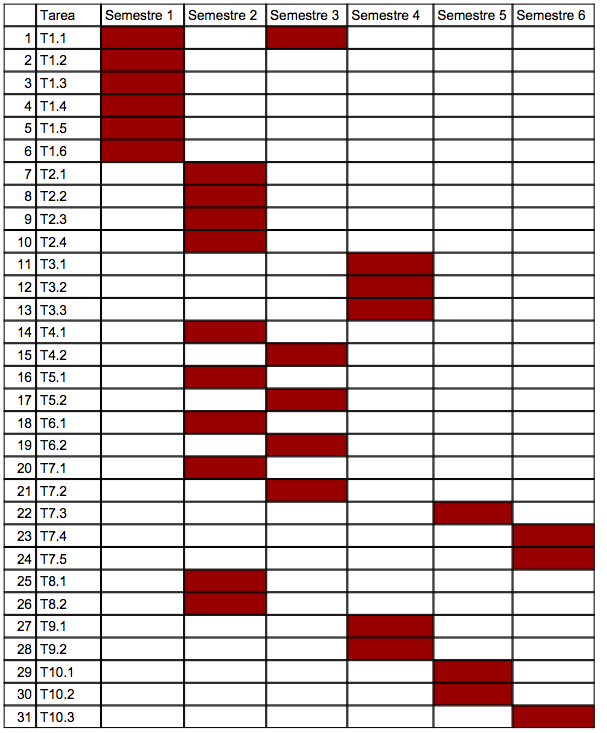
\includegraphics[width=0.80\textwidth]{gantt_chart.png}
\end{center}
\caption{Diagrama de Gantt que resume la repartici\'on de tareas del cronograma (Secci\'on \ref{cronograma}).
\label{gantt}}
\end{figure}

\begin{itemize}
\item[\bf SEM-1]
\begin{itemize}
\item[T1.1] \tecn Compra, instalaci\'on y mantenimiento de 3TB espacio de disco
  con backup para almacenar los datos originales de las simulaciones.
\item[T1.2] \tecn Compra, instalaci\'on y mantenimiento de un blade de
  procesamiento con 24 procesadores con 512GB para poder analizar y
  postprocesar las simulaciones.
\item[T1.4] \gradA\prof Instalaci\'on del software abierto {\texttt N-GenIC}\footnote{\url{http://www.mpa-garching.mpg.de/gadget/}} para la generaci\'on de condiciones iniciales.
\item[T1.3] \gradA\prof Instalaci\'on del software abierto {\texttt
  Gadget2}\footnote{\url{http://www.mpa-garching.mpg.de/gadget/}} para hacer simulaciones de N-cuerpos cosmol\'ogicas.
\item[T1.5] \gradA\prof Instalaci\'on del sofware abierto {\texttt
  Rockstar}\footnote{\url{https://bitbucket.org/gfcstanford/rockstar}} para la detecci\'on de halos de materia oscura.
\item[T1.6] \gradA\gradB\prof Organizaci\'on de una escuela internacional en
  cosmolog\'ia computational (duraci\'on de un mes) para formar
  recurso humano con capacidad de utilizar hardware y software para
  hacer y analizar simulaciones de formaci\'on de estructura a gran
  escala. Dr. Stefan Gottloeber ser\'a uno de los profesores.
\end{itemize}


\item[{\bf SEM 2}]
\begin{itemize}

\item[T4.1] \gradA\prof Escribir software para la generaci\'on de cat\'alogos
  ficticios de galaxias aleatorios (i.e. sin ning\'un tipo de
  clustering). 
\item[T5.1] \prof Escribir software que simule la secuencia de observaci\'on
  de DESI sobre un cat\'alog de galaxias generado aleatoriamente. \bob.
\item[T6.1] \prof Escribir software que simule la asignaci\'on de fibras
  \'opticas sobre un cat\'alog de galaxias generadas aleatoriamente.  \bob.
\item[T7.1] \prof Integrar en la base de c\'odigo de DESI el software para
  preparar cat\'alogos ficticios de galaxias aleatorios. \bob. Viaje a Berkeley por dos semanas. 

\item[T2.1] \gradA Generar las condiciones iniciales para 5 vol\'umenes
  cosmol\'ogicos. 
\item[T2.2] \gradA Correr las simulaciones para 5 vol\'umenes LCDM.
\item[T2.3] \gradA Controlar la calidad de los 5 vol\'umenes LCDM.  
Esto se har\'a con la asesor\'ia de Dr. Stefan Gottloeber.
\item[T2.4] \gradA Identificar los halos de materia oscura en los 5
  vol\'umenes LCDM.
\item[T8.1] \gradB Medir la intensidad del efecto AP sobre cat\'alogos
  ficticios de galaxias creados a partir de simulaciones de N-cuerpos.\park
\item[T8.2] \prof Medir la intensidad del efecto AP sobre observaciones
  reales de galaxias. \park. Viaje a Seul por dos semanas.
\end{itemize}


\item[\bf SEM-3]
\begin{itemize}
\item[T1.1] \tecn Compra, instalaci\'on y mantenimiento de 3TB espacio de disco
  con backup para almacenar los datos originales de las simulaciones.
\item[T4.2] \gradA\prof Adaptar el c\'odigo {\texttt
  make\_survey}\footnote{\url{https://github.com/mockFactory/make_survey}}
  para generar  cat\'alogos fictios de galaxias a partir de
  cat\'alogos de halos materia oscura. 
\item[T5.2] \prof Escribir software que simule la secuencia de observaci\'on
  de DESI sobre un cat\'alogo de galaxias generado a partir de una
  simulaci\'on de N-cuerpos. \bob.
\item[T6.2] \prof Escribir software que simule la asignaci\'on de fibras
  \'opticas sobre un cat\'alog de galaxias generado a partir de una
  simulaci\'on de N-cuerpos. \bob.
\item[T7.2] \gradA\prof Integrar en la base de c\'odigo de DESI el software para
  preparar cat\'alogos ficticios de galaxias a partir de simulaciones
  de N-cuerpos. \bob. Viaje a Berkeley por 2 semanas.
\end{itemize}

\item[\bf SEM-4]
\begin{itemize}
\item[T3.1] \gradA Correr 5 simulaciones $w$CDM para las mismas condiciones 
  iniciales pero diferentes valores de $w$. 
\item[T3.2] \gradA Controlar la calidad de los 5 vol\'umenes $w$CDM. Esto se
  har\'a con la asesor\'ia de Dr. Stefan Gottloeber. 
\item[T3.3] \gradA Identificar los halos de materia oscura en los 5 vol\'umenes $w$CDM. 
\item[T9.1] \gradB\prof Cuantificar el n\'umero de pares de c\'umulos de galaxias  con velocidades extremas en simulaciones de N-cuerpos en
  cosmolog\'ias LCDM. 
\item[T9.2] \gradB Cuantificar el n\'umero de pares de c\'umulos de galaxias con velocidades extremas en simulaciones de N-cuerpos en
  cosmolog\'ias $\omega$CDM. Viaje a Seul por 2 semanas.
\end{itemize}


\item[\bf SEM-5]
\begin{itemize}
\item[T7.3] \prof Integrar en la base de c\'odigo de DESI el software para
  definir las secuencias de observaci\'on del experimento. \bob.
\item[T10.1] \gradB
  Cuantificar el efecto de RSD sobre cat\'alogos ficticios de
  galaxias creados a partir de simulaciones de N-cuerpos en
  cosmolog\'ias LCDM. 
\item[T10.2] \gradB Cuantificar el efecto de RSD sobre cat\'alogos ficticios de
  galaxias creados a partir de simulaciones de N-cuerpos en
  cosmolog\'ias $\omega$CDM. 
\end{itemize}

\item[\bf SEM-6]
\begin{itemize}
\item[T7.4] \prof Integrar el c\'odigo completo de simulaci\'on end-to-end
  de DESI. \bob. 
\item[T7.5] \prof Producir simulaciones completas de simulaci\'on end-to-end
  de DESI. Desde las observaciones hasta la estimaci\'on de redshifts
  de galaxias observadas. \bob. Visita a Berkeley por 2 semanas.
\item[T10.3] \gradB Cuantificar el efecto de RSD sobre los cat\'alogos de
  posiciones y redshift creados a partir de la herramienta de
  simulaci\'on end-to-end de DESI.\bob Visita a Berkely por 2 semanas.
\end{itemize}

\end{itemize}


\section{Impacto ambiental}
%Los proyectos de investigación deben incluir una reflexión
%responsable sobre los efectos positivos o negativos que puedan tener
%sobre el medio natural y la salud humana en el corto, mediano y largo
%plazo. 


\section{Presupuesto}

\begin{table}[h]
\begin{center}
\begin{tabular}{|l|r|r|r|}\hline
\textbf{Rubro} 	& {\bf Financiado} & {\bf Contrapartida} & {\bf Total}\\\hline 
Equipos	& 68.019.081 &	82.824.427 &	150.843.508\\\hline
Bibliografia	&0	&0	&0 \\\hline
Personal científico	&0	&53.264.193	&53.264.193\\\hline
Materiales e insumos	&0	&0	&0\\\hline
Servicios Técnicos	&0	&0	&0\\\hline
Viajes	&51,000,000	&23.000.000	&74.000.000\\\hline
Salidas de Campo	&0	&0	&0\\\hline
Eventos Académicos	&10.000.000	&15.296.367	&25.296.367\\\hline
Publicaciones y patentes&	12.000.000	&4.000.000	&16,000,000\\\hline
Software&	0	&0	&0\\\hline
Gastos de Operación&	14.801.908	&0	&14.801.908\\\hline
Total desembolsado por Colciencias&	162.820.989	&0	&162.820.989\\\hline
Seguimiento y Evaluación&	 4.884.630	&0	&4.884.630\\\hline
Valor total&	{\bf 159.774.619}	& {\bf 178.384.987}	&{\bf 338.159.606}\\\hline

\end{tabular} 
\caption{Resumen Presupuesto. Todos los rubros en COP.}
\end{center}
\label{Resumen Presupuesto}
\end{table}


\begin{table}[h]
\begin{center}
\begin{tabular}{|l|p{5.5cm}|r|r|r|}\hline
{\bf Rubro}	&{\bf Descripción}	& {\bf Año 1}	& {\bf Año 2}	& {\bf Año 3}\\\hline
Viajes	&Visita a Berkeley, Estudiante \#1	&0	&	6.000.000&0\\\hline
Viajes	&Visita a Seoul,  Estudiante\#2	&0	&7.000.000	&0\\\hline
Viajes	&Visita a Berkeley,  Estudiante\#2	&0	&0& 6.000.000 \\\hline
Viajes	&Visita a Berkeley, Profesor	&0	&6.000.000	&6.000.000\\\hline
Viajes	&Presentación Internacional, Estudiante \#1	&0	&5.000.000	&0\\\hline
Viajes	&Presentación Internacional, Estudiante \#2	&0	&0	&5.000.000\\\hline
Viajes	&Presentación Internacional, Profesor	&0	&5.000.000	&5.000.000\\\hline
Publicaciones	&Astrophysical Journal	&0	&6.000.000	&6.000.000\\\hline
Eventos	&Escuela Internacional de Cosmología	&10.000.000	&0	&0\\\hline
Equipos	&Almacenamiento de 6TB con backup 	&19.923.663	&19.923.663	&0\\\hline
Equipos	&Compra de 1 Blade, 24 procesadores y 512GB de RAM 	&28.171.755	&0	&0\\\hline
\multicolumn{2}{|c|}{{\bf Total por año}}	 & 59.095.418	&54.923.663	&28.000.000 \\\hline
\multicolumn{2}{|c|}{\bf Total } & \multicolumn{3}{|c|}{{\bf 148.019.081}}\\\hline
\end{tabular} 
\caption{Desglose del presupuesto de los items financiados por COLCIENCIAS sin incluir gastos de 
operaci\'on y gastos de seguimiento y evaluaci\'on. Todos los rubros en COP.}
\end{center}
\label{Resumen Presupuesto Colciencias}
\end{table}


\begin{table}[h]
\begin{center}
\begin{tabular}{|l|p{3.0cm}|r|r|r|p{2.5cm}|}\hline
{\bf Rubro}	&{\bf Item}	& {\bf Año 1}	& {\bf Año 2}	& {\bf Año 3}	& {\bf Fuente}\\	\hline
Viajes	&Escuela Internacional Estudiante \#1	&5.000.000	&0	&0	&Vicerrectoria investigaciones (FAPA)	\\\hline
Viajes	&Escuela Internacional Estudiante \#2	&5.000.000	&0	&0	&Vicerrectoria investigaciones (FAPA)	\\\hline
Viajes	&Visita a Seoul, Profesor	&7.000.000	&0	&0	&Vicerrectoria investigaciones (FAPA)	\\\hline
Viajes	&Visita a Berkeley, Profesor	&6.000.000	&0	&0	&Vicerrectoria investigaciones (FAPA)	\\\hline
Publicaciones	&Astrophysical Journal	&4.000.000	&0	&0	&Vicerrectoria investigaciones (FAPA)	\\\hline
Personal Científico	&Sueldo Profesor	&17.060.435	&17.746.940	&18.456.818	&Universidad de los Andes\\	\hline
Eventos	&Escuela Internacional de Cosmología	&15.296.367	&0	&0	&Silla Sanford, Departamento de Fisica	\\\hline
Equipos	&Cluster para c\'omputo de alto rendimiento (10\% de la inversion total)	&82.824.427	&0	&0	&Departamento de Servicios de Informacion y Tecnologia\\\hline
\multicolumn{2}{|c|}{{\bf Total por año}}&	142.181.229	&17.746.940	&18.456.818&\\\hline
\multicolumn{2}{|c|}{{\bf Total aportado}}&	 \multicolumn{3}{|c|}{{\bf 178.384.987}}&\\\hline
\end{tabular} 
\caption{Desglose del presupuesto de los items financiados por la Universidad de los Andes
 El sueldo del profesor corresponde a 7 horas/semana, con aumentos de 4\% anuales. Todos los rubros en COP. }
\end{center}
\label{Resumen Presupuesto Colciencias}
\end{table}

\newpage


%Fuentes bibliográficas empleadas en cada uno de los ítems del
%proyecto. Se hará referencia únicamente a aquellas fuentes empleadas
%en el suministro de la información del respectivo proyecto. No se
%incluirán referencias que no se citen. Las citas, en cada uno de los
%campos del formulario, se harán empleando el número de la referencia
%dentro de paréntesis cuadrados (p. ej. [1]). 

\newpage
\bibliography{referencias}{}
\bibliographystyle{plain}


\end{document}
